\chapter{Smart Agriculture and Irrigation}

This chapter reviews concrete smart agriculture and irrigation systems that use sensors, communication networks, controllers, or machine learning to support irrigation decisions. These works are important because they establish the sensing and automation layer required before a complete irrigation digital twin can be built.

\section{Wireless Sensor Network Irrigation}

\subsection[Remote Sensing and Control of an Irrigation System Using a Distributed Wireless Sensor Network]{Remote Sensing and Control of an Irrigation System Using a Distributed Wireless Sensor Network \cite{kim2008wsnIrrigation}}

\subsubsection{Overview}

Kim et al. propose a distributed wireless sensor network for remote sensing and control of an irrigation system. The work addresses the difficulty of monitoring field conditions and controlling irrigation equipment without continuous manual inspection. It is relevant because it connects field sensing with irrigation actuation, which is one of the basic requirements of smart irrigation.

\subsubsection{Architecture / Methodology}

The system is organized around distributed sensor nodes installed in the field. These nodes are responsible for collecting local measurements that describe the irrigation environment. The purpose is to reduce the need for manual inspection and to provide the controller with field information at different locations.

The communication layer connects the distributed nodes to the irrigation control unit. This layer is important because field sensors are useful only if their measurements can be transmitted reliably to the place where irrigation decisions are made. The paper therefore treats wireless communication as a central part of the irrigation architecture.

The control component uses the received data to support remote irrigation operation. In this type of system, the methodological chain is simple but important: collect field data, transmit the data, interpret the measurements, and control the irrigation equipment. This chain is a foundation for later digital twin systems, where the same data would also update a virtual field state.

\begin{figure}[H]
    \centering
    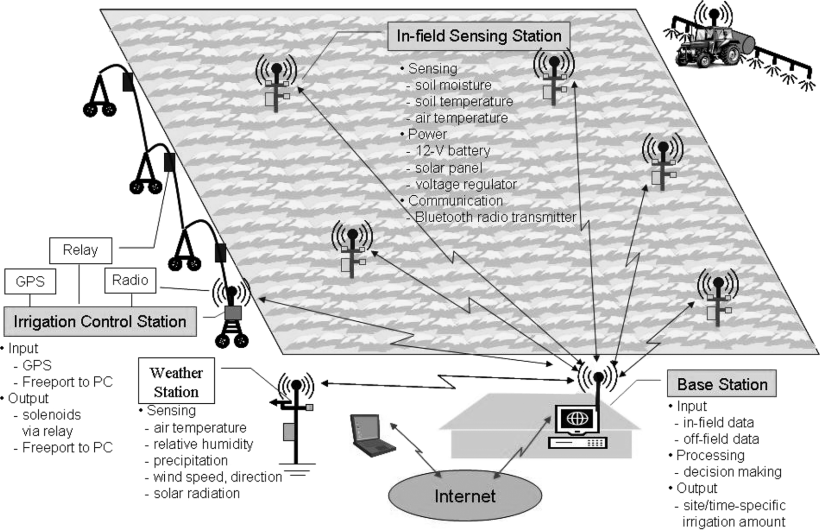
\includegraphics[width=0.75\textwidth]{figures/chapter_04/chapitre 4.1.1.png}
    \caption{Distributed wireless sensor network for remote irrigation sensing and control, adapted from \cite{kim2008wsnIrrigation}. Source: \url{https://doi.org/10.1109/TIM.2008.917198}.}
    \label{fig:soa_kim_wsn_irrigation}
\end{figure}

\subsubsection{Evaluation and Results}

The paper evaluates the system as a practical wireless sensor network and control prototype for irrigation. It demonstrates the feasibility of using distributed sensing for remote irrigation monitoring and control. The verified metadata does not provide exact values for water saving, packet delivery, or crop yield improvement, so this review treats the validation as prototype-based and qualitative.

\subsubsection{Limitations and Relevance to This Project}

The main limitation is that the work is mainly an irrigation monitoring and control system, not a synchronized digital twin with a virtual model and predictive simulation. It is useful because it shows how field sensors and control equipment can be connected in an irrigation context. The remaining gap is to combine this sensing-control loop with virtual representation, prediction, and decision support.

\subsection[Automated Irrigation System Using a Wireless Sensor Network and GPRS Module]{Automated Irrigation System Using a Wireless Sensor Network and GPRS Module \cite{gutierrez2014wsnGprsIrrigation}}

\subsubsection{Overview}

Gutierrez et al. present an automated irrigation system that combines a wireless sensor network with a GPRS communication module. The paper addresses the need for remote operation in agricultural fields where wired communication is difficult or expensive. Its relevance lies in the integration of field sensing, long-range communication, and automatic irrigation control.

\subsubsection{Architecture / Methodology}

The architecture begins with field sensor nodes that collect measurements from the agricultural environment. These nodes form a wireless sensor network, which allows the system to cover a field without wired infrastructure. This is important for agricultural deployment because farms are often spatially distributed and difficult to cable.

The GPRS module extends the communication range. Instead of keeping the system limited to local communication, GPRS allows data to be sent to remote users or services. This makes the irrigation system more suitable for remote supervision and control.

The irrigation actuation layer closes the loop. Measurements collected in the field are transmitted through the network, processed by the control unit, and used to activate or deactivate irrigation. The methodology therefore combines sensing, communication, decision, and actuation in one automated irrigation workflow.

\begin{figure}[H]
    \centering
    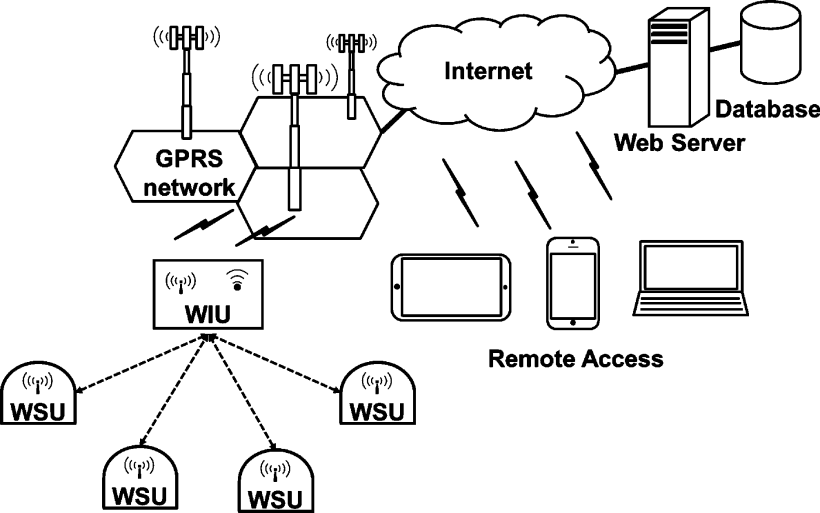
\includegraphics[width=0.75\textwidth]{figures/chapter_04/chapitre 4.1.2.png}
    \caption{Automated irrigation architecture using WSN and GPRS communication, adapted from \cite{gutierrez2014wsnGprsIrrigation}. Source: \url{https://doi.org/10.1109/TIM.2013.2276487}.}
    \label{fig:soa_gutierrez_wsn_gprs}
\end{figure}

\subsubsection{Evaluation and Results}

The work is evaluated as an automated irrigation prototype. It validates that WSN and GPRS technologies can be used to support remote irrigation management. The verified metadata does not expose exact numerical results for water savings, communication reliability, or energy consumption. Therefore, the result is considered qualitative validation of the architecture.

\subsubsection{Limitations and Relevance to This Project}

The limitation is that the system focuses on automation and remote communication, but it does not include a full digital twin layer or advanced prediction. It remains relevant because it demonstrates a practical field-communication pattern for irrigation systems. The gap is to enrich this pattern with real-time virtual state, irrigation simulation, and intelligent recommendation.

\section{Low-Cost IoT Irrigation}

\subsection[A Low Cost Smart Irrigation System Using MQTT Protocol]{A Low Cost Smart Irrigation System Using MQTT Protocol \cite{kodali2017mqttirrigation}}

\subsubsection{Overview}

Kodali and Sarjerao propose a low-cost smart irrigation system using the MQTT protocol. The paper addresses the need for affordable irrigation automation based on lightweight IoT communication. It is relevant because MQTT is widely used in IoT systems where small devices need to publish sensor readings and receive commands.

\subsubsection{Architecture / Methodology}

The methodology is based on a low-cost IoT architecture. A field device collects irrigation-related measurements and communicates them to the application layer. The goal is to make the system affordable while still supporting automatic irrigation decisions.

MQTT is the central communication protocol. It uses a publish-subscribe model, where field devices publish sensor readings and application components subscribe to the topics they need. The same model can also be used to send control commands back to the device. This is useful in irrigation because sensor messages are usually small and frequent.

The control logic connects communication with actuation. Once the application receives the sensor data, it can decide whether the pump or valve should be activated. The paper therefore demonstrates how a lightweight messaging protocol can support a complete sensing-to-control irrigation loop.

\begin{figure}[H]
    \centering
    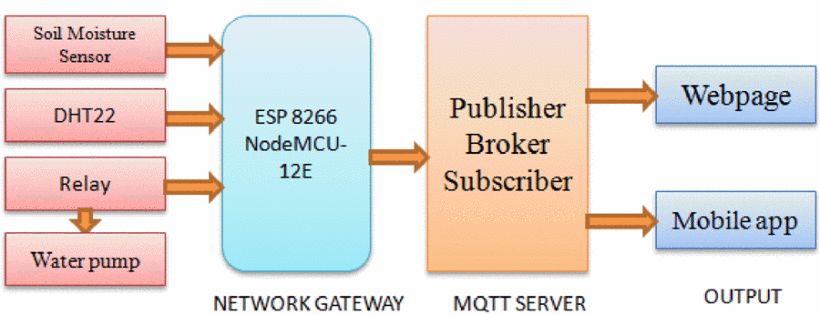
\includegraphics[width=0.75\textwidth]{figures/chapter_04/chapitre 4.2.1.png}
    \caption{Low-cost MQTT-based smart irrigation architecture, adapted from \cite{kodali2017mqttirrigation}. Source: \url{https://doi.org/10.1109/TENCONSpring.2017.8070095}.}
    \label{fig:soa_kodali_mqtt_irrigation}
\end{figure}

\subsubsection{Evaluation and Results}

The paper validates the system as a low-cost prototype. It demonstrates that MQTT can support basic irrigation monitoring and control. The verified metadata does not provide detailed numeric measurements for latency, water saving, or field-scale performance, so the validation is treated as qualitative prototype validation.

\subsubsection{Limitations and Relevance to This Project}

The limitation is that the system is mainly an IoT control prototype. It does not include digital twin synchronization, water-balance simulation, or machine-learning decision support. Its relevance is high at the communication level because MQTT is appropriate for connecting field devices to a backend. The gap is to build a higher-level decision and virtual representation layer on top of the IoT communication.

\section{Machine Learning for Irrigation Decision Support}

\subsection[An IoT Based Smart Irrigation Management System Using Machine Learning and Open Source Technologies]{An IoT Based Smart Irrigation Management System Using Machine Learning and Open Source Technologies \cite{goap2018iotMLIrrigation}}

\subsubsection{Overview}

Goap et al. propose an IoT-based smart irrigation management system that uses machine learning and open-source technologies. The problem addressed is the improvement of irrigation decisions by combining sensed data with learning-based prediction. This work is relevant because it moves beyond rule-based irrigation and introduces data-driven decision support.

\subsubsection{Architecture / Methodology}

The methodology combines IoT sensing with machine-learning decision support. The IoT layer collects data from the agricultural environment. These data may include soil and environmental variables that influence crop water needs. The data are then sent to a processing layer where they can be cleaned, organized, and prepared for decision-making.

The machine-learning layer is the main difference between this work and simpler rule-based irrigation systems. Instead of relying only on fixed thresholds, the system uses learned relationships between input variables and irrigation decisions. This allows the decision process to consider several variables together.

The application layer presents or applies the irrigation decision. In this workflow, the system moves from sensing to data processing, then to prediction or classification, and finally to irrigation management. The use of open-source technologies makes the architecture easier to reproduce and adapt.

For a digital twin project, this methodology is important because machine learning can become part of the virtual decision layer. However, a digital twin still needs a synchronized virtual representation in addition to prediction.

\begin{figure}[H]
    \centering
    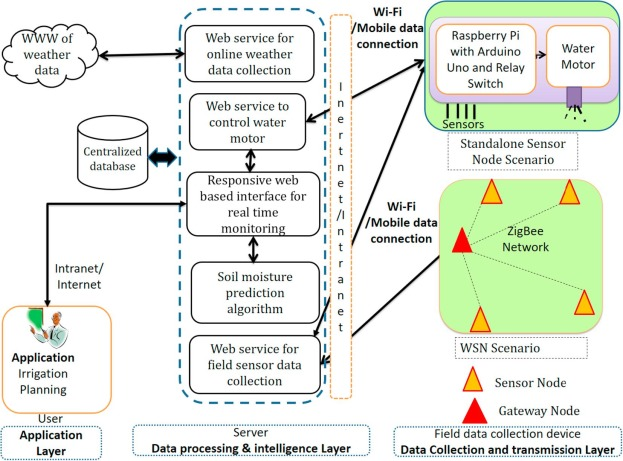
\includegraphics[width=0.65\textwidth]{figures/chapter_04/chapitre 4.3.1.jpg}
    \caption{IoT and machine-learning workflow for smart irrigation management, adapted from \cite{goap2018iotMLIrrigation}. Source: \url{https://doi.org/10.1016/j.compag.2018.09.040}.}
    \label{fig:soa_goap_iot_ml_irrigation}
\end{figure}

\subsubsection{Evaluation and Results}

The paper evaluates the proposed smart irrigation management system as an IoT and machine-learning implementation. It demonstrates that machine learning can be integrated with open-source IoT components for irrigation decision support. The verified metadata does not provide exact performance values for prediction accuracy, water saving, or yield improvement. Therefore, this review describes the result as implementation validation rather than a confirmed field-scale performance benchmark.

\subsubsection{Limitations and Relevance to This Project}

The limitation is that the paper focuses on smart irrigation decision support, not on a complete digital twin with continuous physical-virtual synchronization. It is useful because it shows how machine learning can be placed between sensor data and irrigation decisions. The remaining gap is to connect this decision layer to a virtual representation of the field and to a real-time monitoring and control workflow.

\section{Discussion}

The selected smart irrigation papers show that soil and environmental sensing, wireless communication, and automation are already practical in irrigation systems. Wireless sensor networks and GPRS make field monitoring possible over distributed areas. MQTT provides a lightweight IoT communication model. Machine learning adds the possibility of data-driven irrigation decisions. However, these systems usually remain at the level of monitoring, control, or decision support. They do not fully model a synchronized virtual copy of the irrigation system, and they rarely combine sensing, prediction, simulation, user decision support, and actuation into one complete digital twin.

\begingroup
\scriptsize
\setlength{\tabcolsep}{1pt}
\begin{longtable}{@{}>{\raggedright\arraybackslash}p{0.12\textwidth}>{\raggedright\arraybackslash}p{0.12\textwidth}>{\raggedright\arraybackslash}p{0.13\textwidth}>{\raggedright\arraybackslash}p{0.12\textwidth}>{\raggedright\arraybackslash}p{0.15\textwidth}>{\raggedright\arraybackslash}p{0.11\textwidth}>{\raggedright\arraybackslash}p{0.12\textwidth}>{\raggedright\arraybackslash}p{0.12\textwidth}@{}}
\caption{Comparison of selected smart irrigation papers}\\
\toprule
Paper & Application & Sensors / data & Communication & Irrigation decision method & Validation & Main result & Limitation \\
\midrule
\endfirsthead
\toprule
Paper & Application & Sensors / data & Communication & Irrigation decision method & Validation & Main result & Limitation \\
\midrule
\endhead
Kim et al. \cite{kim2008wsnIrrigation} & Remote irrigation sensing and control & Distributed field measurements & Wireless sensor network & Control based on sensed field data & Prototype & Shows feasibility of remote sensing and control & No digital twin or predictive simulation \\
Gutierrez et al. \cite{gutierrez2014wsnGprsIrrigation} & Automated irrigation & Field sensor-node data & WSN and GPRS & Automated controller using sensor data & Prototype & Demonstrates remote automated irrigation architecture & Limited virtual modeling and AI support \\
Kodali and Sarjerao \cite{kodali2017mqttirrigation} & Low-cost smart irrigation & IoT sensor readings & MQTT & Lightweight publish-subscribe control logic & Prototype & Shows MQTT suitability for low-cost irrigation IoT & Basic control without digital twin layer \\
Goap et al. \cite{goap2018iotMLIrrigation} & Smart irrigation management & IoT and environmental data & IoT network & Machine-learning decision support & Implementation & Integrates ML with open-source IoT irrigation & No full physical-virtual synchronization \\
\bottomrule
\end{longtable}
\endgroup

The synthesis of gaps is clear. Smart irrigation systems already handle sensing, connectivity, and automation, but they often lack a persistent virtual model of the field state. They also tend to treat irrigation as a direct control problem rather than as a digital twin problem where the physical field, virtual representation, prediction layer, and decision workflow are synchronized.
